% !TEX root = scientific-computing.tex

% this needs to be at the top of each file with the \plot command and the word in the [] is the session for pythontex. 
\begin{jlcode}[plots]
using Plots, PGFPlotsX
pgfplotsx()
\end{jlcode}


\chapter{Plotting Data and Functions}\label{chapter-11-plotting-data-and-functions}


Plotting is crucial to understanding functions and visualizing data.
There are many ways to do some plots using various packages. Instead of covering details of multiple packages, we will cover the Plots package, which is overlay over many other plotting packages.  

\hypertarget{the-plots-package}{%
\section{The Plots Package}\label{the-plots-package}}

There is a relatively simple, but powerful plotting package called
\texttt{Plots} and don't forget to download it as in Appendix \ref{ch:packages}. The full documentation
is at \href{http://docs.juliaplots.org/latest/}{the Plots.jl website}.
Recall that once the package is added, enter \jlb[plots]{using Plots}


The Plots package tries to unify the syntax for plotting anything. The
basic command for plotting data or functions in 2D is the \texttt{plot}
command. The idea call \texttt{plot} on any type of object that can be plotted. The next few examples shows this.


\subsection{Plotting Functions}

For plotting a function, simply call plot on the function: 
\begin{jlblock}[plots]
plot(x->x^2)
\end{jlblock}
%
produces the following plot: 
\begin{center}
\pgfplotsset{scale=0.5}
\plot{plots/plots/plot01.tex}{plots}
\end{center}
Note: your plot may look a bit different than this one with different fonts.  This is mainly due to using a different backend, which is explained below. 

If you want to specify the $x$-range, try: \jlb[plots]{plot(x->x^2,-2,2)} which generates: 
\begin{center}
\pgfplotsset{scale=0.5}
\plot{plots/plots/plot01a.tex}{plots}
\end{center}

If we want to plot 2 or more functions on the same axes, pass in an array of functions like: 
\begin{jlblock}[plots]
plot([x->x^2,x->sin(x)],-2,2)
\end{jlblock}
%
produces the following:
\begin{center}
\pgfplotsset{scale=0.5}
\plot{plots/plots/plot02.tex}{plots}
\end{center}

We will also see below how to change other aspects of the plot including the legend, title, labels on the axes, etc.  


\subsection{Plotting Data}

First, let's start with some random data. Let

\begin{jlblock}[plots]
x=1:10
y=rand(1:10,10)
\end{jlblock}
%
then \jlb[plots]{plot(x,y)} will produce a scatter plot of the data, like
%
\begin{center}
\pgfplotsset{scale=0.7}
\plot{plots/plots/plot03.tex}{plots}
\end{center}
%
and note that since these are just random points, your plot will look
different, but the style should be the same.

If we want to connect all of the points with points instead, type
%
\begin{jlblock}[plots]
plot(x,y,seriestype=:scatter)
\end{jlblock}
%
and the plot will look like:

\begin{center}
\pgfplotsset{scale=0.7}
\plot{plots/plots/plot04.tex}{plots}
\end{center}

There is a shorthand or different version of this: \jlv[plots]{scatter(x,y)}, which produces the same plot. 
If you want both, then type

\begin{jlblock}[plots]
plot(x,y,seriestype=[:scatter,:line])
\end{jlblock}
%
\begin{center}
\pgfplotsset{scale=0.7}
\plot{plots/plots/plot05.tex}{plots}
\end{center}


\section{Backends of the Plots package}

The \texttt{Plots.jl} package actually doesn't do the plotting. It
leaves the details to other packages. By default, \texttt{Plots} uses the \texttt{GR}
backend although in this text I have used the \texttt{PGFPlotsX} backend. There
are a number of backends that you may want to try. The standard ones
are:

\begin{itemize}
\item  PyPlot (matplotlib): Slow but dependable
\item  GR: Feature-rich and fast, but new
\item  Plotly/PlotlyJS: Interactive and good for web
\item  PGFPlotsX: Native LaTeX rendering
\item  UnicodePlots: Plots to unicode for situations without graphics
  capabilities.
\end{itemize}

To switch the backend, you type the backend name in all lowercase with a set of (). Note:
you will need to add and load the package. Here is the plot of $x^2$ on various backends.

\begin{jlverbatim}
gr()
plot(x->x^2,-2,2)
\end{jlverbatim}
gives:
%
\begin{center}
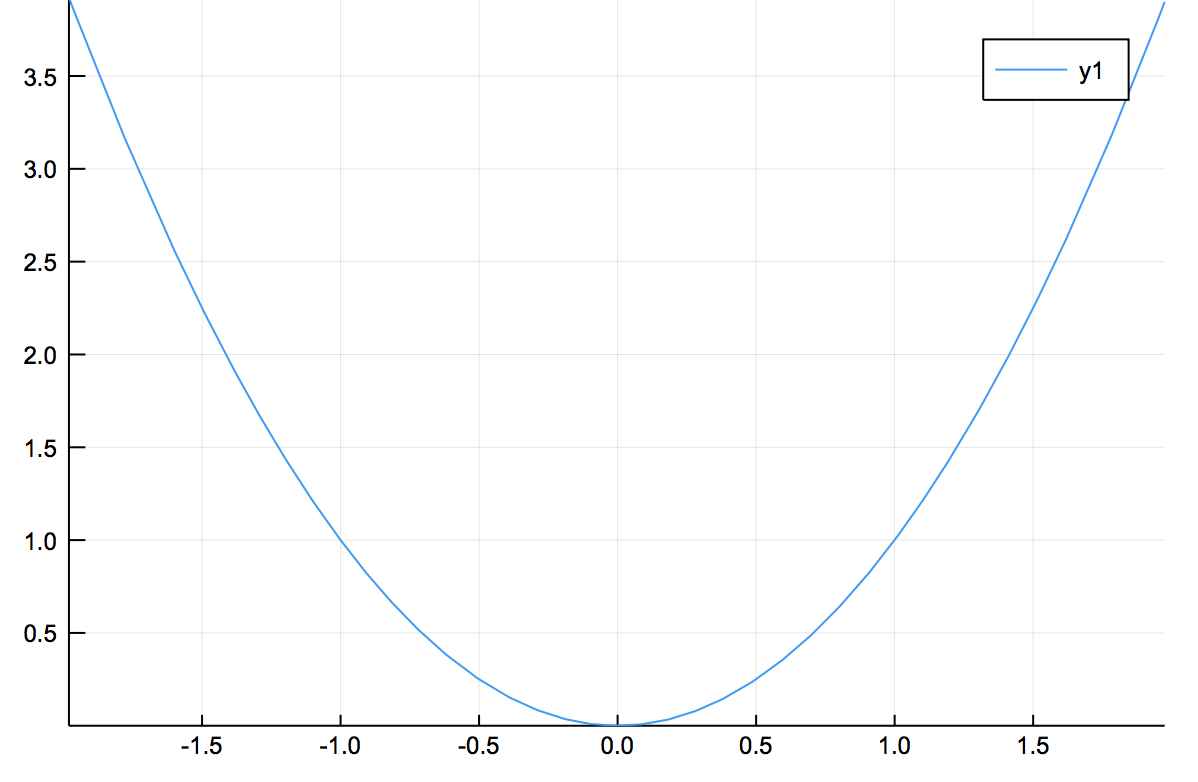
\includegraphics[width=4in]{plots/plots/plot08.png}
\end{center}

\begin{jlverbatim}
using PlotlyJS
plotlyjs()
plot(x->x^2,-2,2)
\end{jlverbatim}
%
results in:
%
\begin{center}
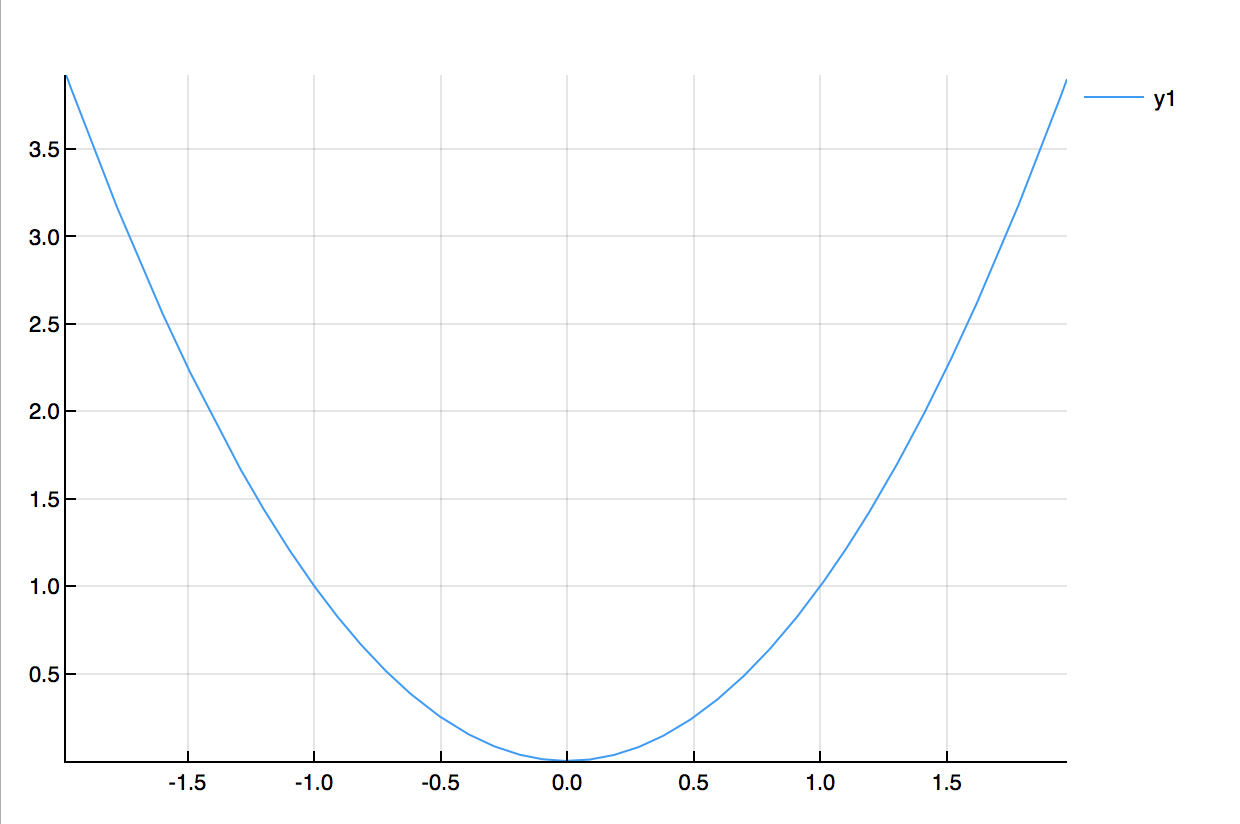
\includegraphics[width=4in]{plots/plots/plot09.png}
\end{center}
and then

\begin{jlblock}[plots]
using PGFPlotsX
pgfplotsx()
plot(x->x^2,-2,2)
\end{jlblock}
%
results in:
%
\begin{center}
\pgfplotsset{scale=0.6}
\plot{plots/plots/pgfplotsx.tex}{plots}
\end{center}
and finally
%
\begin{jlverbatim}
using PyPlot
pyplot()
plot(x->x^2,-2,2)
\end{jlverbatim}
%
results in:
%
\begin{center}
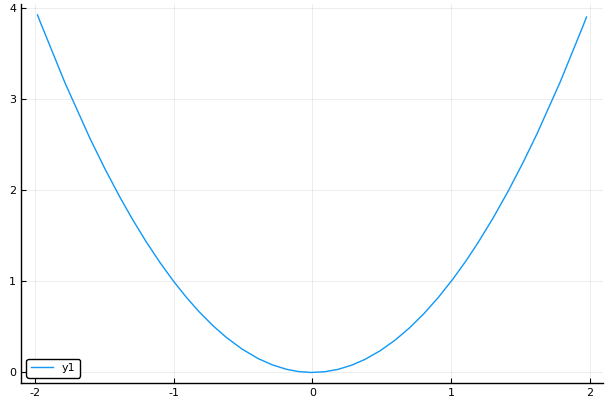
\includegraphics[width=4in]{plots/plots/plot11.png}
\end{center}

For additional information on the supported backends, visit
\href{http://docs.juliaplots.org/latest/backends/}{the Plots.jl backend
documentation}


\subsection{Changing the attributes of the plot}

Let's return back to the function plots above (although this works for
point/line plots as well) and change many attributes of the curve. As an
example:

\begin{jlblock}[plots]
plot([x->x^2,sin],-2,2,title="Two Curves",label=["x squared" "sin(x)"],xlabel="x",ylabel="y",lw=3)
\end{jlblock}

results in
%
\begin{center}
\pgfplotsset{scale=0.7}
\plot{plots/plots/attrs.tex}{plots}
\end{center}
The format is fairly clear for the changing of the attributes. Note: in
this example:

\begin{itemize}
\item  the \texttt{title} changes the title of the plot
\item  the \texttt{label} changes the legend.
\item  the \texttt{xlabel} and \texttt{ylabel} changes the axes labels.
\item  the \texttt{lw} is the line weight.
\end{itemize}

To avoid duplicating tons of documentation, visit
\href{http://docs.juliaplots.org/latest/attributes/}{the Plots.jl page
on attributes} to find all of the information to get the plot the way
you want. 

\subsection{Exercise}

\begin{itemize}

\item  Take the scatterplot above (with the random dots) and change the color
  of the dots to darkgreen, change the markers to diamonds and the size of the points 
  to about twice the default size.
\item On the function plot, make the line thicker and style to dashed. 
\end{itemize}


\section{Other plots}

\subsection{Parametric Plots}

To do a parametric plot, like the circle defined by $x(t)=\cos t, y(t)=\sin t$, then

\begin{jlblock}[plots]
plot(t->cos(t),t->sin(t),0,2*pi,legend=false)
\end{jlblock}
%
where the legend is turned off, since with one curve, it doesn't make much sense. The result is
\begin{center}
\pgfplotsset{scale=0.7}
\plot{plots/plots/parametric01.tex}{plots}
\end{center}


but notice that this should be a circle, but it looks like an ellipse
due to the aspect ratio. If one instead adds the
\verb!aspect_ratio=:equal! option, as in 
\begin{jlblock}[plots]
plot(t->cos(t),t->sin(t),0,2*pi,aspect_ratio=:equal, legend=false)
\end{jlblock}
\begin{center}
\pgfplotsset{scale=0.7}
\plot{plots/plots/parametric02.tex}{plots}
\end{center}


\subsection{Bar plots}

A bar plot can be made with the \texttt{bar} command. For example:

\begin{jlblock}[plots]
bar(1:10,y)
\end{jlblock}
where y was defined above for the scatter plot.  The result is
%
\begin{center}
\pgfplotsset{scale=0.7}
\plot{plots/plots/bar01.tex}{plots}
\end{center}


\subsection{Surface Plots}

If we have a function of 2 variables, a surface plot is nice to use. For
example, if we have the function \(f(x,y)=0.1e^{x^2+y^2}\) and we want
to plot it from -3 to 3 in both directions, if we define

\begin{jlblock}[plots]
f(x,y)=exp(-0.1*(x^2+y^2))
x = y = range(-5, stop = 5, length = 40)
\end{jlblock}
%
and then plot with
%
\begin{jlverbatim}
plot(x,y, f, st = :surface)
\end{jlverbatim}


\begin{jlcode}[plots]
pl = plot(x,y, f, st = :surface)

function cleanPreamble(preamble::String)
  lines_to_remove = r"RequirePackage|documentclass|usepackage|compat=newest|usepgfplotslibrary|^%\sDefault|usetikzlibrary"
  split(preamble,"\n") |> arr -> filter(str -> !occursin(lines_to_remove,str),arr) |> arr -> join(arr,"\n")
end

open("plots/plots/surf_preamble.tex", "w") do io
           write(io, cleanPreamble(Plots.pgfx_preamble(pl)))
       end;

\end{jlcode}


\begin{center}
\pgfplotsset{scale=0.7}
\IfFileExists{./plots/plots/surf_preamble.tex}{\input{plots/plots/surf_preamble.tex}}{}
%\plot{plots/plots/surf.tex}{plots}
{\color{red} HIDDEN PLOT}
\end{center}


\subsection{Heat maps}

Similar to above, we can make a heat map with

\begin{jlverbatim}
plot(x,y, f, st=:heatmap)
\end{jlverbatim}

\begin{jlcode}[plots]
pl = plot(x,y, f, st=:heatmap)

open("plots/plots/heat_preamble.tex", "w") do io
           write(io, cleanPreamble(Plots.pgfx_preamble(pl)))
       end;
\end{jlcode}
%
which produces
%
\begin{center}
\pgfplotsset{scale=0.7}
\IfFileExists{./plots/plots/heat_preamble.tex}{\pgfplotsset{%
layers/standard/.define layer set={%
    background,axis background,axis grid,axis ticks,axis lines,axis tick labels,pre main,main,axis descriptions,axis foreground%
}{grid style= {/pgfplots/on layer=axis grid},%
    tick style= {/pgfplots/on layer=axis ticks},%
    axis line style= {/pgfplots/on layer=axis lines},%
    label style= {/pgfplots/on layer=axis descriptions},%
    legend style= {/pgfplots/on layer=axis descriptions},%
    title style= {/pgfplots/on layer=axis descriptions},%
    colorbar style= {/pgfplots/on layer=axis descriptions},%
    ticklabel style= {/pgfplots/on layer=axis tick labels},%
    axis background@ style={/pgfplots/on layer=axis background},%
    3d box foreground style={/pgfplots/on layer=axis foreground},%
    },
}

\pgfplotsset{
colormap={plots1}{rgb(0.00000000cm)=(0.00146200,0.00046600,0.01386600)
rgb(0.00392157cm)=(0.00226700,0.00127000,0.01857000)
rgb(0.00784314cm)=(0.00329900,0.00224900,0.02423900)
rgb(0.01176471cm)=(0.00454700,0.00339200,0.03090900)
rgb(0.01568627cm)=(0.00600600,0.00469200,0.03855800)
rgb(0.01960784cm)=(0.00767600,0.00613600,0.04683600)
rgb(0.02352941cm)=(0.00956100,0.00771300,0.05514300)
rgb(0.02745098cm)=(0.01166300,0.00941700,0.06346000)
rgb(0.03137255cm)=(0.01399500,0.01122500,0.07186200)
rgb(0.03529412cm)=(0.01656100,0.01313600,0.08028200)
rgb(0.03921569cm)=(0.01937300,0.01513300,0.08876700)
rgb(0.04313725cm)=(0.02244700,0.01719900,0.09732700)
rgb(0.04705882cm)=(0.02579300,0.01933100,0.10593000)
rgb(0.05098039cm)=(0.02943200,0.02150300,0.11462100)
rgb(0.05490196cm)=(0.03338500,0.02370200,0.12339700)
rgb(0.05882353cm)=(0.03766800,0.02592100,0.13223200)
rgb(0.06274510cm)=(0.04225300,0.02813900,0.14114100)
rgb(0.06666667cm)=(0.04691500,0.03032400,0.15016400)
rgb(0.07058824cm)=(0.05164400,0.03247400,0.15925400)
rgb(0.07450980cm)=(0.05644900,0.03456900,0.16841400)
rgb(0.07843137cm)=(0.06134000,0.03659000,0.17764200)
rgb(0.08235294cm)=(0.06633100,0.03850400,0.18696200)
rgb(0.08627451cm)=(0.07142900,0.04029400,0.19635400)
rgb(0.09019608cm)=(0.07663700,0.04190500,0.20579900)
rgb(0.09411765cm)=(0.08196200,0.04332800,0.21528900)
rgb(0.09803922cm)=(0.08741100,0.04455600,0.22481300)
rgb(0.10196078cm)=(0.09299000,0.04558300,0.23435800)
rgb(0.10588235cm)=(0.09870200,0.04640200,0.24390400)
rgb(0.10980392cm)=(0.10455100,0.04700800,0.25343000)
rgb(0.11372549cm)=(0.11053600,0.04739900,0.26291200)
rgb(0.11764706cm)=(0.11665600,0.04757400,0.27232100)
rgb(0.12156863cm)=(0.12290800,0.04753600,0.28162400)
rgb(0.12549020cm)=(0.12928500,0.04729300,0.29078800)
rgb(0.12941176cm)=(0.13577800,0.04685600,0.29977600)
rgb(0.13333333cm)=(0.14237800,0.04624200,0.30855300)
rgb(0.13725490cm)=(0.14907300,0.04546800,0.31708500)
rgb(0.14117647cm)=(0.15585000,0.04455900,0.32533800)
rgb(0.14509804cm)=(0.16268900,0.04355400,0.33327700)
rgb(0.14901961cm)=(0.16957500,0.04248900,0.34087400)
rgb(0.15294118cm)=(0.17649300,0.04140200,0.34811100)
rgb(0.15686275cm)=(0.18342900,0.04032900,0.35497100)
rgb(0.16078431cm)=(0.19036700,0.03930900,0.36144700)
rgb(0.16470588cm)=(0.19729700,0.03840000,0.36753500)
rgb(0.16862745cm)=(0.20420900,0.03763200,0.37323800)
rgb(0.17254902cm)=(0.21109500,0.03703000,0.37856300)
rgb(0.17647059cm)=(0.21794900,0.03661500,0.38352200)
rgb(0.18039216cm)=(0.22476300,0.03640500,0.38812900)
rgb(0.18431373cm)=(0.23153800,0.03640500,0.39240000)
rgb(0.18823529cm)=(0.23827300,0.03662100,0.39635300)
rgb(0.19215686cm)=(0.24496700,0.03705500,0.40000700)
rgb(0.19607843cm)=(0.25162000,0.03770500,0.40337800)
rgb(0.20000000cm)=(0.25823400,0.03857100,0.40648500)
rgb(0.20392157cm)=(0.26481000,0.03964700,0.40934500)
rgb(0.20784314cm)=(0.27134700,0.04092200,0.41197600)
rgb(0.21176471cm)=(0.27785000,0.04235300,0.41439200)
rgb(0.21568627cm)=(0.28432100,0.04393300,0.41660800)
rgb(0.21960784cm)=(0.29076300,0.04564400,0.41863700)
rgb(0.22352941cm)=(0.29717800,0.04747000,0.42049100)
rgb(0.22745098cm)=(0.30356800,0.04939600,0.42218200)
rgb(0.23137255cm)=(0.30993500,0.05140700,0.42372100)
rgb(0.23529412cm)=(0.31628200,0.05349000,0.42511600)
rgb(0.23921569cm)=(0.32261000,0.05563400,0.42637700)
rgb(0.24313725cm)=(0.32892100,0.05782700,0.42751100)
rgb(0.24705882cm)=(0.33521700,0.06006000,0.42852400)
rgb(0.25098039cm)=(0.34150000,0.06232500,0.42942500)
rgb(0.25490196cm)=(0.34777100,0.06461600,0.43021700)
rgb(0.25882353cm)=(0.35403200,0.06692500,0.43090600)
rgb(0.26274510cm)=(0.36028400,0.06924700,0.43149700)
rgb(0.26666667cm)=(0.36652900,0.07157900,0.43199400)
rgb(0.27058824cm)=(0.37276800,0.07391500,0.43240000)
rgb(0.27450980cm)=(0.37900100,0.07625300,0.43271900)
rgb(0.27843137cm)=(0.38522800,0.07859100,0.43295500)
rgb(0.28235294cm)=(0.39145300,0.08092700,0.43310900)
rgb(0.28627451cm)=(0.39767400,0.08325700,0.43318300)
rgb(0.29019608cm)=(0.40389400,0.08558000,0.43317900)
rgb(0.29411765cm)=(0.41011300,0.08789600,0.43309800)
rgb(0.29803922cm)=(0.41633100,0.09020300,0.43294300)
rgb(0.30196078cm)=(0.42254900,0.09250100,0.43271400)
rgb(0.30588235cm)=(0.42876800,0.09479000,0.43241200)
rgb(0.30980392cm)=(0.43498700,0.09706900,0.43203900)
rgb(0.31372549cm)=(0.44120700,0.09933800,0.43159400)
rgb(0.31764706cm)=(0.44742800,0.10159700,0.43108000)
rgb(0.32156863cm)=(0.45365100,0.10384800,0.43049800)
rgb(0.32549020cm)=(0.45987500,0.10608900,0.42984600)
rgb(0.32941176cm)=(0.46610000,0.10832200,0.42912500)
rgb(0.33333333cm)=(0.47232800,0.11054700,0.42833400)
rgb(0.33725490cm)=(0.47855800,0.11276400,0.42747500)
rgb(0.34117647cm)=(0.48478900,0.11497400,0.42654800)
rgb(0.34509804cm)=(0.49102200,0.11717900,0.42555200)
rgb(0.34901961cm)=(0.49725700,0.11937900,0.42448800)
rgb(0.35294118cm)=(0.50349300,0.12157500,0.42335600)
rgb(0.35686275cm)=(0.50973000,0.12376900,0.42215600)
rgb(0.36078431cm)=(0.51596700,0.12596000,0.42088700)
rgb(0.36470588cm)=(0.52220600,0.12815000,0.41954900)
rgb(0.36862745cm)=(0.52844400,0.13034100,0.41814200)
rgb(0.37254902cm)=(0.53468300,0.13253400,0.41666700)
rgb(0.37647059cm)=(0.54092000,0.13472900,0.41512300)
rgb(0.38039216cm)=(0.54715700,0.13692900,0.41351100)
rgb(0.38431373cm)=(0.55339200,0.13913400,0.41182900)
rgb(0.38823529cm)=(0.55962400,0.14134600,0.41007800)
rgb(0.39215686cm)=(0.56585400,0.14356700,0.40825800)
rgb(0.39607843cm)=(0.57208100,0.14579700,0.40636900)
rgb(0.40000000cm)=(0.57830400,0.14803900,0.40441100)
rgb(0.40392157cm)=(0.58452100,0.15029400,0.40238500)
rgb(0.40784314cm)=(0.59073400,0.15256300,0.40029000)
rgb(0.41176471cm)=(0.59694000,0.15484800,0.39812500)
rgb(0.41568627cm)=(0.60313900,0.15715100,0.39589100)
rgb(0.41960784cm)=(0.60933000,0.15947400,0.39358900)
rgb(0.42352941cm)=(0.61551300,0.16181700,0.39121900)
rgb(0.42745098cm)=(0.62168500,0.16418400,0.38878100)
rgb(0.43137255cm)=(0.62784700,0.16657500,0.38627600)
rgb(0.43529412cm)=(0.63399800,0.16899200,0.38370400)
rgb(0.43921569cm)=(0.64013500,0.17143800,0.38106500)
rgb(0.44313725cm)=(0.64626000,0.17391400,0.37835900)
rgb(0.44705882cm)=(0.65236900,0.17642100,0.37558600)
rgb(0.45098039cm)=(0.65846300,0.17896200,0.37274800)
rgb(0.45490196cm)=(0.66454000,0.18153900,0.36984600)
rgb(0.45882353cm)=(0.67059900,0.18415300,0.36687900)
rgb(0.46274510cm)=(0.67663800,0.18680700,0.36384900)
rgb(0.46666667cm)=(0.68265600,0.18950100,0.36075700)
rgb(0.47058824cm)=(0.68865300,0.19223900,0.35760300)
rgb(0.47450980cm)=(0.69462700,0.19502100,0.35438800)
rgb(0.47843137cm)=(0.70057600,0.19785100,0.35111300)
rgb(0.48235294cm)=(0.70650000,0.20072800,0.34777700)
rgb(0.48627451cm)=(0.71239600,0.20365600,0.34438300)
rgb(0.49019608cm)=(0.71826400,0.20663600,0.34093100)
rgb(0.49411765cm)=(0.72410300,0.20967000,0.33742400)
rgb(0.49803922cm)=(0.72990900,0.21275900,0.33386100)
rgb(0.50196078cm)=(0.73568300,0.21590600,0.33024500)
rgb(0.50588235cm)=(0.74142300,0.21911200,0.32657600)
rgb(0.50980392cm)=(0.74712700,0.22237800,0.32285600)
rgb(0.51372549cm)=(0.75279400,0.22570600,0.31908500)
rgb(0.51764706cm)=(0.75842200,0.22909700,0.31526600)
rgb(0.52156863cm)=(0.76401000,0.23255400,0.31139900)
rgb(0.52549020cm)=(0.76955600,0.23607700,0.30748500)
rgb(0.52941176cm)=(0.77505900,0.23966700,0.30352600)
rgb(0.53333333cm)=(0.78051700,0.24332700,0.29952300)
rgb(0.53725490cm)=(0.78592900,0.24705600,0.29547700)
rgb(0.54117647cm)=(0.79129300,0.25085600,0.29139000)
rgb(0.54509804cm)=(0.79660700,0.25472800,0.28726400)
rgb(0.54901961cm)=(0.80187100,0.25867400,0.28309900)
rgb(0.55294118cm)=(0.80708200,0.26269200,0.27889800)
rgb(0.55686275cm)=(0.81223900,0.26678600,0.27466100)
rgb(0.56078431cm)=(0.81734100,0.27095400,0.27039000)
rgb(0.56470588cm)=(0.82238600,0.27519700,0.26608500)
rgb(0.56862745cm)=(0.82737200,0.27951700,0.26175000)
rgb(0.57254902cm)=(0.83229900,0.28391300,0.25738300)
rgb(0.57647059cm)=(0.83716500,0.28838500,0.25298800)
rgb(0.58039216cm)=(0.84196900,0.29293300,0.24856400)
rgb(0.58431373cm)=(0.84670900,0.29755900,0.24411300)
rgb(0.58823529cm)=(0.85138400,0.30226000,0.23963600)
rgb(0.59215686cm)=(0.85599200,0.30703800,0.23513300)
rgb(0.59607843cm)=(0.86053300,0.31189200,0.23060600)
rgb(0.60000000cm)=(0.86500600,0.31682200,0.22605500)
rgb(0.60392157cm)=(0.86940900,0.32182700,0.22148200)
rgb(0.60784314cm)=(0.87374100,0.32690600,0.21688600)
rgb(0.61176471cm)=(0.87800100,0.33206000,0.21226800)
rgb(0.61568627cm)=(0.88218800,0.33728700,0.20762800)
rgb(0.61960784cm)=(0.88630200,0.34258600,0.20296800)
rgb(0.62352941cm)=(0.89034100,0.34795700,0.19828600)
rgb(0.62745098cm)=(0.89430500,0.35339900,0.19358400)
rgb(0.63137255cm)=(0.89819200,0.35891100,0.18886000)
rgb(0.63529412cm)=(0.90200300,0.36449200,0.18411600)
rgb(0.63921569cm)=(0.90573500,0.37014000,0.17935000)
rgb(0.64313725cm)=(0.90939000,0.37585600,0.17456300)
rgb(0.64705882cm)=(0.91296600,0.38163600,0.16975500)
rgb(0.65098039cm)=(0.91646200,0.38748100,0.16492400)
rgb(0.65490196cm)=(0.91987900,0.39338900,0.16007000)
rgb(0.65882353cm)=(0.92321500,0.39935900,0.15519300)
rgb(0.66274510cm)=(0.92647000,0.40538900,0.15029200)
rgb(0.66666667cm)=(0.92964400,0.41147900,0.14536700)
rgb(0.67058824cm)=(0.93273700,0.41762700,0.14041700)
rgb(0.67450980cm)=(0.93574700,0.42383100,0.13544000)
rgb(0.67843137cm)=(0.93867500,0.43009100,0.13043800)
rgb(0.68235294cm)=(0.94152100,0.43640500,0.12540900)
rgb(0.68627451cm)=(0.94428500,0.44277200,0.12035400)
rgb(0.69019608cm)=(0.94696500,0.44919100,0.11527200)
rgb(0.69411765cm)=(0.94956200,0.45566000,0.11016400)
rgb(0.69803922cm)=(0.95207500,0.46217800,0.10503100)
rgb(0.70196078cm)=(0.95450600,0.46874400,0.09987400)
rgb(0.70588235cm)=(0.95685200,0.47535600,0.09469500)
rgb(0.70980392cm)=(0.95911400,0.48201400,0.08949900)
rgb(0.71372549cm)=(0.96129300,0.48871600,0.08428900)
rgb(0.71764706cm)=(0.96338700,0.49546200,0.07907300)
rgb(0.72156863cm)=(0.96539700,0.50224900,0.07385900)
rgb(0.72549020cm)=(0.96732200,0.50907800,0.06865900)
rgb(0.72941176cm)=(0.96916300,0.51594600,0.06348800)
rgb(0.73333333cm)=(0.97091900,0.52285300,0.05836700)
rgb(0.73725490cm)=(0.97259000,0.52979800,0.05332400)
rgb(0.74117647cm)=(0.97417600,0.53678000,0.04839200)
rgb(0.74509804cm)=(0.97567700,0.54379800,0.04361800)
rgb(0.74901961cm)=(0.97709200,0.55085000,0.03905000)
rgb(0.75294118cm)=(0.97842200,0.55793700,0.03493100)
rgb(0.75686275cm)=(0.97966600,0.56505700,0.03140900)
rgb(0.76078431cm)=(0.98082400,0.57220900,0.02850800)
rgb(0.76470588cm)=(0.98189500,0.57939200,0.02625000)
rgb(0.76862745cm)=(0.98288100,0.58660600,0.02466100)
rgb(0.77254902cm)=(0.98377900,0.59384900,0.02377000)
rgb(0.77647059cm)=(0.98459100,0.60112200,0.02360600)
rgb(0.78039216cm)=(0.98531500,0.60842200,0.02420200)
rgb(0.78431373cm)=(0.98595200,0.61575000,0.02559200)
rgb(0.78823529cm)=(0.98650200,0.62310500,0.02781400)
rgb(0.79215686cm)=(0.98696400,0.63048500,0.03090800)
rgb(0.79607843cm)=(0.98733700,0.63789000,0.03491600)
rgb(0.80000000cm)=(0.98762200,0.64532000,0.03988600)
rgb(0.80392157cm)=(0.98781900,0.65277300,0.04558100)
rgb(0.80784314cm)=(0.98792600,0.66025000,0.05175000)
rgb(0.81176471cm)=(0.98794500,0.66774800,0.05832900)
rgb(0.81568627cm)=(0.98787400,0.67526700,0.06525700)
rgb(0.81960784cm)=(0.98771400,0.68280700,0.07248900)
rgb(0.82352941cm)=(0.98746400,0.69036600,0.07999000)
rgb(0.82745098cm)=(0.98712400,0.69794400,0.08773100)
rgb(0.83137255cm)=(0.98669400,0.70554000,0.09569400)
rgb(0.83529412cm)=(0.98617500,0.71315300,0.10386300)
rgb(0.83921569cm)=(0.98556600,0.72078200,0.11222900)
rgb(0.84313725cm)=(0.98486500,0.72842700,0.12078500)
rgb(0.84705882cm)=(0.98407500,0.73608700,0.12952700)
rgb(0.85098039cm)=(0.98319600,0.74375800,0.13845300)
rgb(0.85490196cm)=(0.98222800,0.75144200,0.14756500)
rgb(0.85882353cm)=(0.98117300,0.75913500,0.15686300)
rgb(0.86274510cm)=(0.98003200,0.76683700,0.16635300)
rgb(0.86666667cm)=(0.97880600,0.77454500,0.17603700)
rgb(0.87058824cm)=(0.97749700,0.78225800,0.18592300)
rgb(0.87450980cm)=(0.97610800,0.78997400,0.19601800)
rgb(0.87843137cm)=(0.97463800,0.79769200,0.20633200)
rgb(0.88235294cm)=(0.97308800,0.80540900,0.21687700)
rgb(0.88627451cm)=(0.97146800,0.81312200,0.22765800)
rgb(0.89019608cm)=(0.96978300,0.82082500,0.23868600)
rgb(0.89411765cm)=(0.96804100,0.82851500,0.24997200)
rgb(0.89803922cm)=(0.96624300,0.83619100,0.26153400)
rgb(0.90196078cm)=(0.96439400,0.84384800,0.27339100)
rgb(0.90588235cm)=(0.96251700,0.85147600,0.28554600)
rgb(0.90980392cm)=(0.96062600,0.85906900,0.29801000)
rgb(0.91372549cm)=(0.95872000,0.86662400,0.31082000)
rgb(0.91764706cm)=(0.95683400,0.87412900,0.32397400)
rgb(0.92156863cm)=(0.95499700,0.88156900,0.33747500)
rgb(0.92549020cm)=(0.95321500,0.88894200,0.35136900)
rgb(0.92941176cm)=(0.95154600,0.89622600,0.36562700)
rgb(0.93333333cm)=(0.95001800,0.90340900,0.38027100)
rgb(0.93725490cm)=(0.94868300,0.91047300,0.39528900)
rgb(0.94117647cm)=(0.94759400,0.91739900,0.41066500)
rgb(0.94509804cm)=(0.94680900,0.92416800,0.42637300)
rgb(0.94901961cm)=(0.94639200,0.93076100,0.44236700)
rgb(0.95294118cm)=(0.94640300,0.93715900,0.45859200)
rgb(0.95686275cm)=(0.94690300,0.94334800,0.47497000)
rgb(0.96078431cm)=(0.94793700,0.94931800,0.49142600)
rgb(0.96470588cm)=(0.94954500,0.95506300,0.50786000)
rgb(0.96862745cm)=(0.95174000,0.96058700,0.52420300)
rgb(0.97254902cm)=(0.95452900,0.96589600,0.54036100)
rgb(0.97647059cm)=(0.95789600,0.97100300,0.55627500)
rgb(0.98039216cm)=(0.96181200,0.97592400,0.57192500)
rgb(0.98431373cm)=(0.96624900,0.98067800,0.58720600)
rgb(0.98823529cm)=(0.97116200,0.98528200,0.60215400)
rgb(0.99215686cm)=(0.97651100,0.98975300,0.61676000)
rgb(0.99607843cm)=(0.98225700,0.99410900,0.63101700)
rgb(1.00000000cm)=(0.98836200,0.99836400,0.64492400)},
}
}{}
%\plot{plots/plots/heat.tex}{plots}
{\color{red} HIDDEN PLOT}
\end{center}


\subsection{Animation}

Another nice type of plot under Plots.jl is that of an animation,
however you will need to have \texttt{ffmpeg} installed on your machine.
If you then do

\begin{jlverbatim}
@gif for a in range(0.5,stop=2,length=16)
  plot(t->cos(2t),t->sin(a*t),0,2pi,legend=false)
end
\end{jlverbatim}

which saves to a gif that the output will describe this results in:



\section{Other Plots and subplots}

This just is the tip of the iceberg for plotting. Take a look at the
\href{http://docs.juliaplots.org/latest/}{Plots.jl documentation} or do
some google-foo with the phrase `Plots.jl' and what you're looking for
and good spot for Q\&A is
\href{https://discourse.julialang.org/c/domain/viz}{a julialang.org
discourse site}

\section{Exercises}

Use the plotting techniques in this section to plot the following.  For each, hide the legend when ther e is only one curve/set of data and label appropriate if more than one curve/set of data.  Include a title as well. 

\begin{enumerate}
\item The function $y=e^{-x^2}$ from $x=-3$ to $x=3$
\item The functions $y=\sin x, y=\sin 2x, y=\sin 3$ from $x=-\pi$ to $x=\pi$. 
\item A scatter plot of the following:
\begin{center}
\begin{tabular}{r|rrrrrrrrrrrrrr}
$x$ & 0 & 2 & 3 & 4 & 6 & 9 & 10 & 11 & 13 & 15 & 16 & 18 & 20 \\
$y$ & $-1$ & 4 & 3 & 6 & 2 & 0 & 2 & 9 & 5 & $-2$ & 4 & 6 & 3\\
\end{tabular}
\end{center}
\item A surface plot of $z=\sin(x-y)$ with $0 \leq x \leq \pi, 0 \leq y \leq \pi$.
\item A heat map of $z=\sin(x-y)$ with $0 \leq x \leq \pi, 0 \leq y \leq \pi$.
\end{enumerate}
